 % -*- root: ../../twm.tex -*-
\section[intro]{Motivation}

\begin{frame}
    \frametitle{Rise of Unstructured Data}

\begin{center}
\raisebox{-7pt}{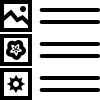
\includegraphics[height=0.8cm]{img/icons/content}}  $\,\!\quad$ instead of $\,\!\quad$  \raisebox{-7pt}{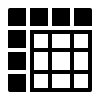
\includegraphics[height=0.8cm]{img/icons/table}} 
\end{center}

\begin{itemize}
    \item Text, speech, images, video
\end{itemize}
\begin{itemize}
    \item \textcolor{iseblue}{Merrill Lynch (1998)}: 80 - 90\% of data is unstructured
\end{itemize}

\begin{itemize}
    \item \textcolor{iseblue}{Gantz and Reinsel (2012)}
    \begin{itemize}
        \item $<$ 1\% of data is analyzed
        \item 40 zettabytes in 2020 (1 ZB = 1 billion TB)
    \end{itemize}
\end{itemize}

\begin{itemize}
    \item Implicit structure
    \begin{itemize}
        \item Text: punctuation, part of speech
        \item Images: coordinates, colors
    \end{itemize}
\end{itemize}

\end{frame}

\begin{frame}[plain]
\hspace*{-32pt}
    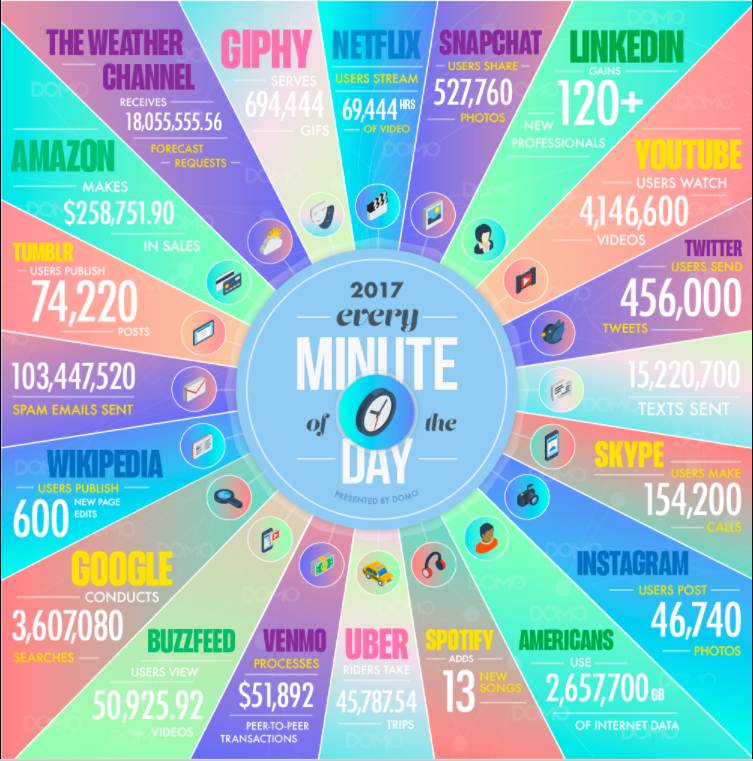
\includegraphics[height=\paperheight]{img/figures/data_never_sleeps}
\vspace{-40pt}
\begin{flushright}
Source \\
\textcolor{iseblue}{\href{https://www.domo.com/learn/data-never-sleeps-5?aid=ogsm072517_1&sf100871281=1}{domo.com}}
\end{flushright}
\end{frame}

\begin{frame}
    \frametitle{One fits All?}
\begin{minipage}[t]{\textwidth}
\begin{minipage}[c]{.3\textwidth}
        \resizebox{.8\textwidth}{!}{\textcolor{isered}{\textbf{How to}}}
\end{minipage}%
\begin{minipage}[c]{.2\textwidth}
    {\Large
        obtain \\[0.4\baselineskip]
        process \\[0.4\baselineskip]
        model \\[0.4\baselineskip]
        interpret \\[0.4\baselineskip]
    }
\end{minipage}%
\begin{minipage}[c]{.2\textwidth}
        \resizebox{.8\textwidth}{!}{\textcolor{isered}{\textbf{texts}}}
\end{minipage}%
\begin{minipage}[c]{.2\textwidth}
        \resizebox{.7\textwidth}{!}{\textcolor{isered}{\textbf{?}}}
\end{minipage}
\end{minipage} \\
\vspace{20pt}
Depends on domain and question.
\end{frame}

\begin{frame}
    \frametitle{Sentiment Pipeline}
    \scalebox{0.78}{
         % -*- root: FSS3.tex -*-
 \label{flowchart}
\begin{tikzpicture}[node distance=2cm]
\node (articles) [doc] {\hyperlink{lab:articles}{Articles}};
\node (scraping) [standard, right of=articles, xshift=0.7cm] {\hyperlink{lab:scraping}{Scraping}};
\node (nlp) [standard, right of=scraping, xshift=0.5cm] {\hyperlink{lab:nlp}{NLP}};
\node (projection) [standard, right of=nlp, xshift=0.7cm] {\hyperlink{lab:projection}{Projection}};

\node (sentiment) [doc, right of=projection, xshift=1.2cm] {Sentiment};

\node[bigbox, below of=scraping, yshift=-0.7cm, xshift=-1.3cm](outbox)
{
%    \begin{minipage}{1.5cm}
%    \center
%        \tikz{\node[box]{\scriptsize URL};}
%        \tikz{\node[box, yshift=1cm]{\scriptsize Author};}
%        \tikz{\node[box]{\scriptsize Symbol};}
%        \tikz{\node[box]{\scriptsize Date};}
%        \tikz{\node[box]{\scriptsize Text};}
%    \end{minipage}

    \begin{minipage}{1.5cm}
    \center
    \begin{tikzpicture}[node distance=0.55cm]
    \node (url) [box] {\scriptsize URL};
    \node (author) [box, below of=url] {\scriptsize Author};
    \node (symbol) [box, below of=author] {\scriptsize Symbol};
    \node (date) [box, below of=symbol] {\scriptsize Date};
    \node (text) [box, below of=date] {\scriptsize Text};
    \end{tikzpicture}
    \end{minipage}
};

\node (nasdaq) [doc, below of=scraping, xshift=-1.3cm, yshift=-3cm] {\hyperlink{lab:articles}{Nasdaq Articles}};
\node (rdc) [below of=scraping, xshift=-1.3cm, yshift=-4cm] {
\href{http://sfb649.wiwi.hu-berlin.de/fedc/index.php}{
\includegraphics[scale=0.18]{img/logos/rdc}}

};

\node (rdc2) [below of=scraping, xshift=-1.3cm, yshift=-4cm] {};

\node[bigbox, below of=nlp, yshift=-0.25cm](outbox2)
{
%    \begin{minipage}{1.5cm}
%    \center
%        \tikz{\node[box]{\scriptsize URL};}
%        \tikz{\node[box, yshift=1cm]{\scriptsize Author};}
%        \tikz{\node[box]{\scriptsize Symbol};}
%        \tikz{\node[box]{\scriptsize Date};}
%        \tikz{\node[box]{\scriptsize Text};}
%    \end{minipage}

    \begin{minipage}{1.6cm}
    \center
    \begin{tikzpicture}[node distance=0.55cm]
    \node (token) [box2] {\scriptsize Token};
    \node (negation) [box2, below of=token] {\scriptsize Negation};
    \node (pos) [box2, below of=negation] {\scriptsize POS};
    \node (lemmatization) [box2, below of=pos] {\scriptsize Lemmata};
    \end{tikzpicture}
    \end{minipage}
};
%\node (nasdaq) [standard, below of=articles, yshift=5cm] {Scraping};

\node[bigbox, below of=projection, yshift=-0.30cm, xshift=1.3cm](outbox3)
{
%    \begin{minipage}{1.5cm}
%    \center
%        \tikz{\node[box]{\scriptsize URL};}
%        \tikz{\node[box, yshift=1cm]{\scriptsize Author};}
%        \tikz{\node[box]{\scriptsize Symbol};}
%        \tikz{\node[box]{\scriptsize Date};}
%        \tikz{\node[box]{\scriptsize Text};}
%    \end{minipage}

    \begin{minipage}{2cm}
    \center
    \begin{tikzpicture}[node distance=0.55cm]
    \node [box3, yshift=0.80cm]{\scriptsize Unsupervised};
    \node (bl) [box2] {\scriptsize BL};
    \node (lm) [box2, below of=token] {\scriptsize LM};
    \end{tikzpicture}
    \end{minipage}
};

\node[bigbox2, below of=projection, yshift=-2.5cm, xshift=1.3cm](outbox4)
{
%    \begin{minipage}{1.5cm}
%    \center
%        \tikz{\node[box]{\scriptsize URL};}
%        \tikz{\node[box, yshift=1cm]{\scriptsize Author};}
%        \tikz{\node[box]{\scriptsize Symbol};}
%        \tikz{\node[box]{\scriptsize Date};}
%        \tikz{\node[box]{\scriptsize Text};}
%    \end{minipage}

    \begin{minipage}{2cm}
    \center
    \begin{tikzpicture}[node distance=0.55cm]
    \node [box3, yshift=0.80cm]{\scriptsize Supervised};
    \node (sm) [box2] {\scriptsize SM};
    \end{tikzpicture}
    \end{minipage}
};

\node[box3, below of=sentiment, yshift=0.5cm, xshift=0.4cm](happy2){
};
\node[box3, below of=sentiment, yshift=0.5cm, xshift=0.6cm](happy){
    
\includegraphics[width=15pt]{img/icons/happy}
};

\node[box3, below of=sentiment, yshift=-0.2cm, xshift=0.4cm](neutral2){
};
\node[box3, below of=sentiment, yshift=-0.2cm, xshift=0.6cm](neutral){
    
\includegraphics[width=15pt]{img/icons/neutral}
};

\node[box3, below of=sentiment, yshift=-0.9cm, xshift=0.4cm](sad2){
};
\node[box3, below of=sentiment, yshift=-0.9cm, xshift=0.6cm](sad){
    
\includegraphics[width=15pt]{img/icons/sad}
};


\draw [arrow] (articles) -- (scraping);
\draw [arrow] (scraping) -- (nlp);
\draw [arrow] (nlp) -- (projection);
\draw [arrow] (projection) -- (sentiment);
\draw [line width=0.25mm] (scraping) |- (outbox);
\draw [line width=0.25mm] (nlp) -- (outbox2);
\draw [arrow] (outbox) -- (nasdaq);
\draw [arrow] (nasdaq) -- (rdc2);
\draw [line width=0.25mm] (projection) |- (outbox3);
\draw [line width=0.25mm] (projection) |- (outbox4);
\draw [line width=0.25mm] (sentiment) |- (happy2);
\draw [line width=0.25mm] (sentiment) |- (neutral2);
\draw [line width=0.25mm] (sentiment) |- (sad2);

%\node (in1) [doc, below of=start] {Input};
%\node (pro1) [process, below of=in1] {Process 1};
%\node (dec1) [decision, below of=pro1] {Decision 1};
\end{tikzpicture}
    }
\end{frame}